\documentclass{beamer}

\usepackage[romanian]{babel}
\usepackage{graphicx}
\usepackage{hyperref}

\title{Gena Pisicii Portocalii}
\author{Anamaria Hodivoianu}
\date{\today}

\begin{document}

\begin{frame}
    \titlepage
\end{frame}

\begin{frame}{Introducere}
    \begin{itemize}
        \item Gena care le da pisicilor portocalii culoarea blanii a fost mult timp un mister
        \item Pisicile portocalii sunt in mare parte masculi, in timp ce pisicile calico si pisicile tortoiseshell sunt in mare parte femele
    \end{itemize}
    \vspace{0.1cm}
    \centering
    \begin{minipage}{0.3\textwidth}
        \centering
        \includegraphics[height=4cm]{orange-tabby-cat-783x1024.jpg}
        \small Pisica Portocalie
    \end{minipage}
    \begin{minipage}{0.3\textwidth}
        \centering
        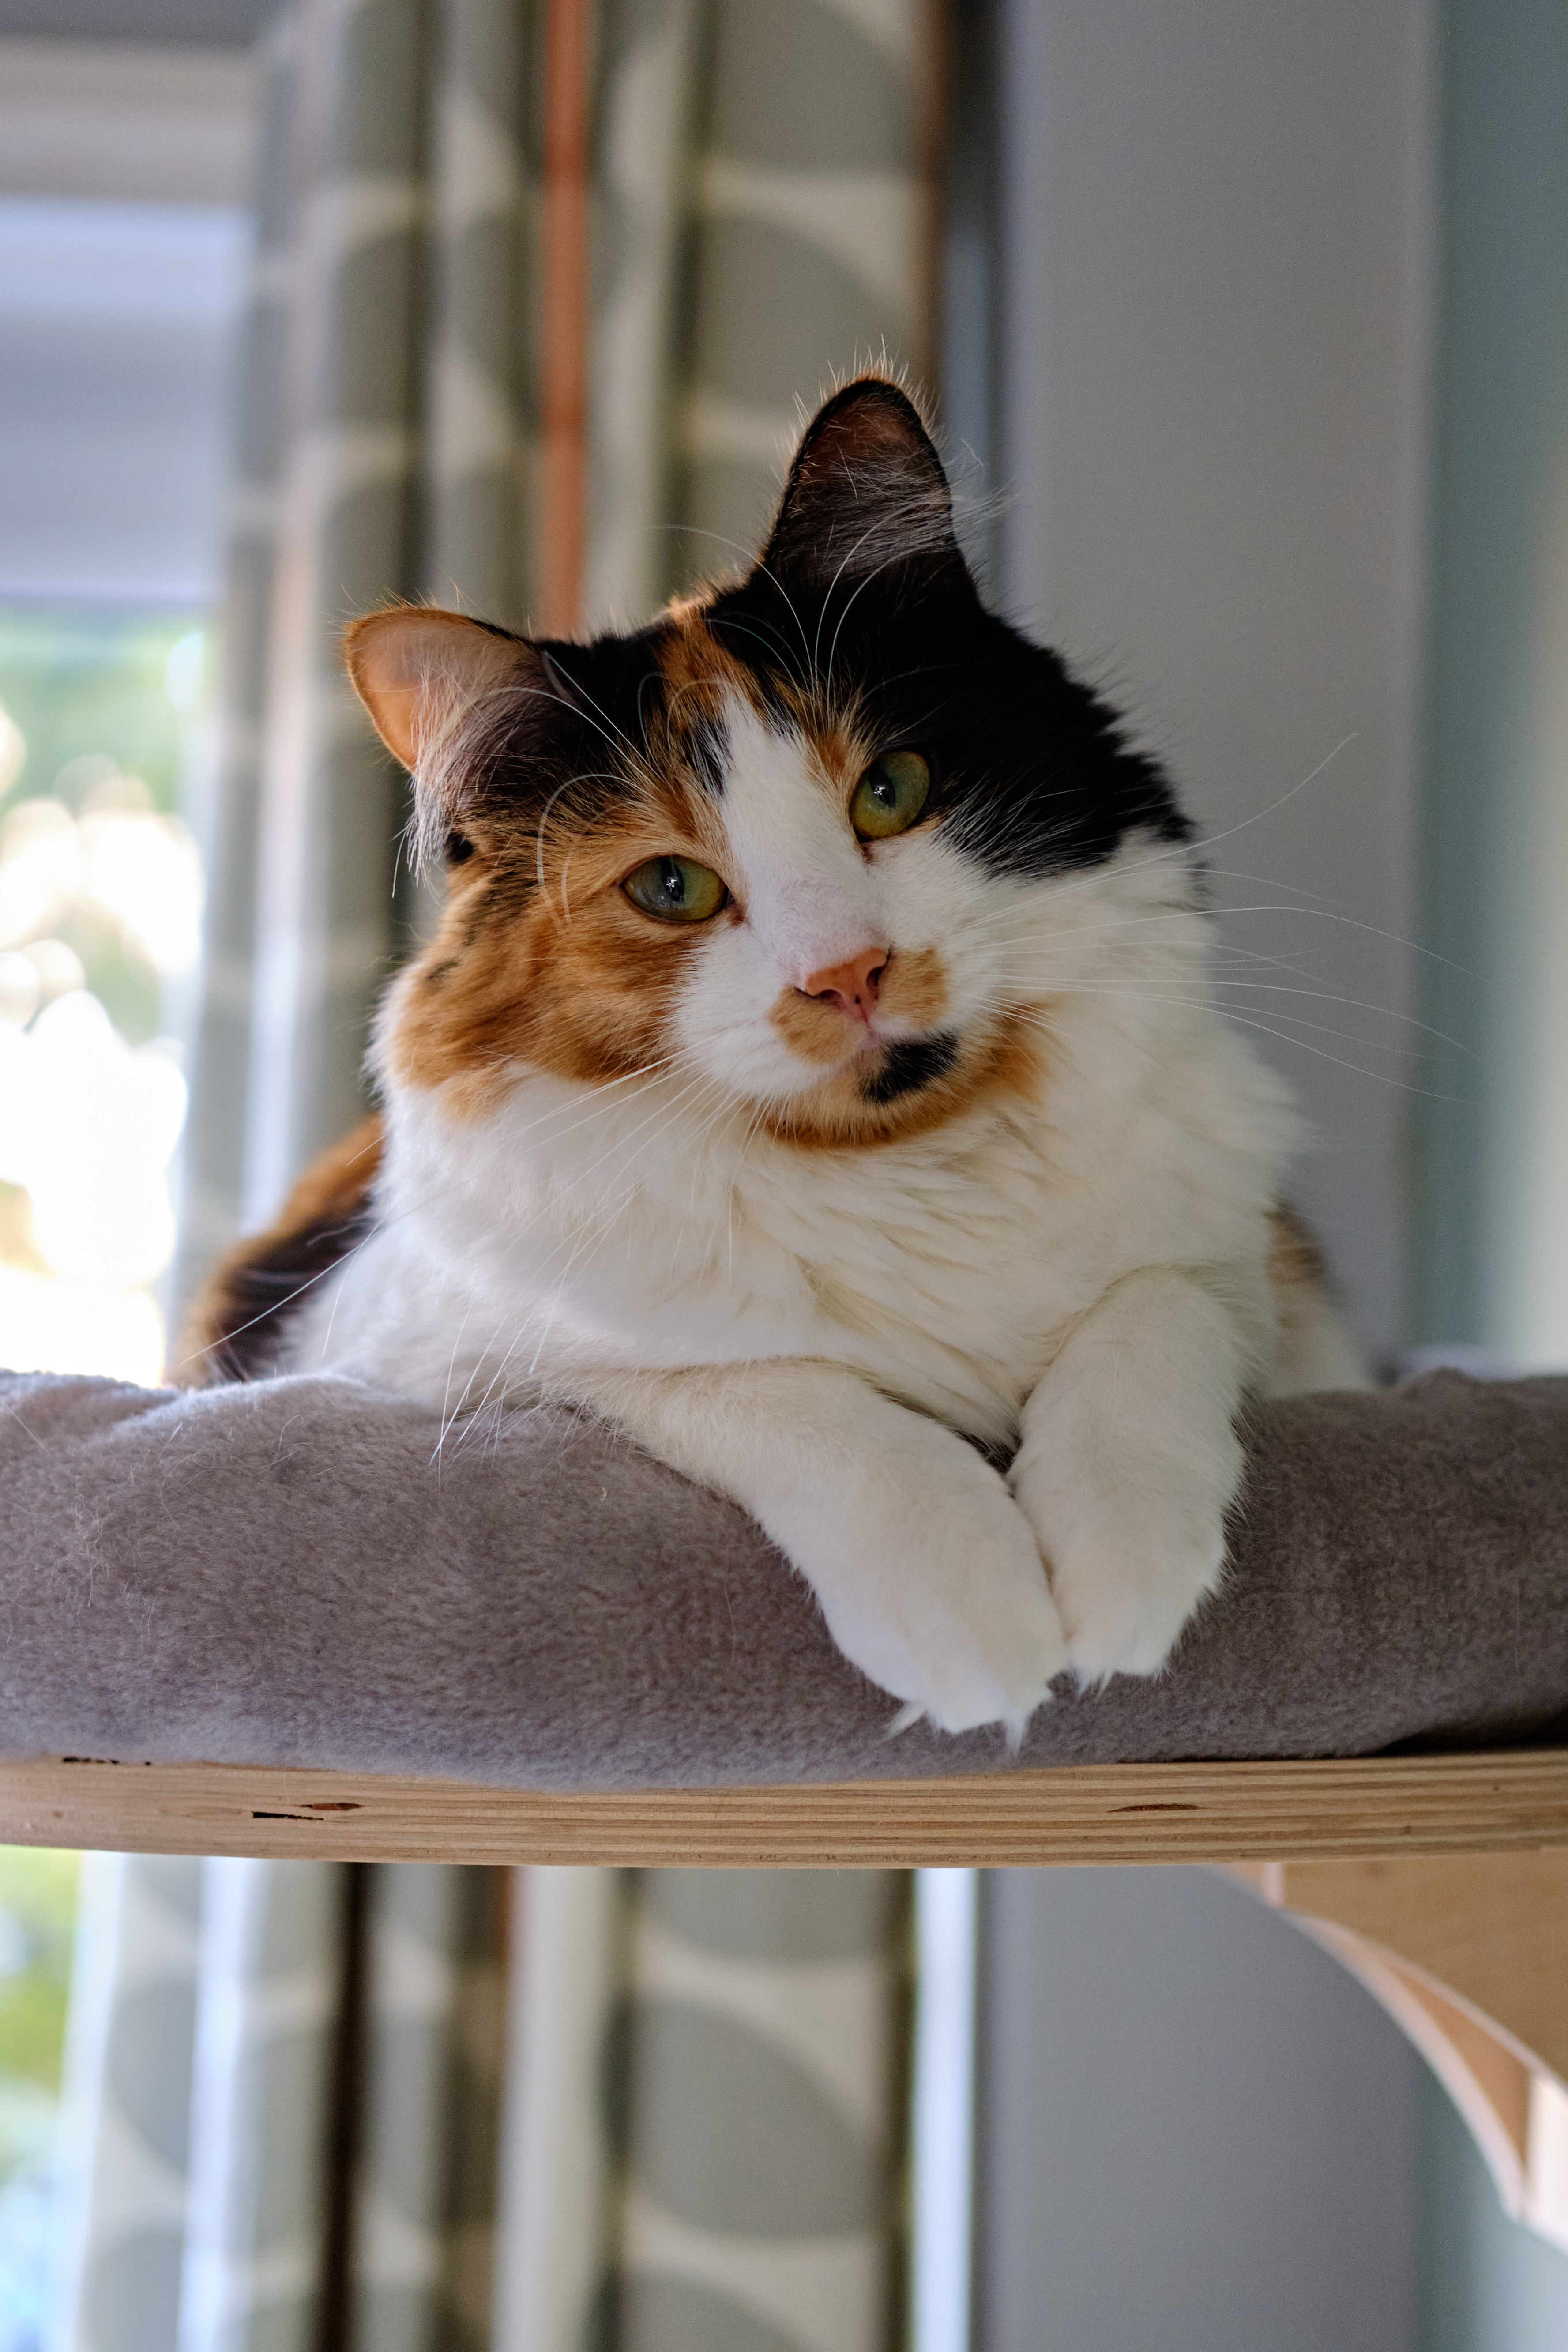
\includegraphics[height=4cm]{A_Calico_cat.jpg}
        \small Pisica Calico
    \end{minipage}
    \hfill
    \begin{minipage}{0.3\textwidth}
        \centering
        \includegraphics[height=4cm]{Short-haired_tortoiseshell_cat.jpg}
        \small Pisica Tortoiseshell
    \end{minipage}
\end{frame}

\begin{frame}{Gena Portocalie}
    \begin{itemize}
        \item Gena responsabila pentru culoarea portocalie a blanii este pe cromozomul X
    \end{itemize}
    \centering
    \begin{minipage}{0.5\textwidth}
        \centering
        \includegraphics[height=6cm]{x-chromosomes.jpg}
    \end{minipage}
\end{frame}

\begin{frame}{Gena Portocalie la Majoritatea Mamiferelor}
    \begin{itemize}
        \item Proteina Mc1r
        \item Gena care o codifica nu se afla pe cromozomul X
        \item La pisicile portocalii nu se gaseste mutatia care cauzeaza parul rosu la alte mamifere
    \end{itemize}
    \centering
    \begin{minipage}{0.6\textwidth}
        \centering
        \includegraphics[height=4cm]{cat-breathing-fast-orange-kitten.jpg}
    \end{minipage}
\end{frame}

\begin{frame}{Gena Portocalie la Pisici}
    \begin{itemize}
        \item Cercetatori de la Stanford, condusi de Dr. Greg Barsh
        \item Melancocite (celule de piele) - pisicile portocalii produc de 13 ori mai mult ARN care codifica gena Arhgap36 decat pisicile fara blana portocalie
        \item Mutatia nu este in gena insasi, ci intr-o alta parte a ADN-ului care influenteaza cantitatea de ARN produsa
        \item Toate pisicile portocalii, calico si tortoiseshell au aceasta mutatie
    \end{itemize}
\end{frame}

\begin{frame}{Gena Portocalie la Pisici}
    \begin{itemize}
        \item Cercetatori de la Kyushu, condusi de Dr. Hiroyuki Sasaki
        \item La pisicile Calico, regiunile cu blana portocalie produc mai mult ARN care codifica gena Arhgap36 decat celelalte regiuni
    \end{itemize}
    \centering
    \begin{minipage}{0.6\textwidth}
        \centering
        \includegraphics[height=4cm]{maxresdefault.jpg}
    \end{minipage}
\end{frame}

\begin{frame}{Concluzii}
    \begin{itemize}
        \item Mutatia care da culoarea portocalie pisicilor a fost descoperita
        \item Se afla pe cromozomul X
        \item Pisicile portocalii produc mai mult ARN care codifica gena Arhgap36   
    \end{itemize}
    \centering
    \begin{minipage}{0.5\textwidth}
        \centering
        \includegraphics[height=4cm]{orange-cat.jpg}
    \end{minipage}
\end{frame}

\begin{frame}
    \centering
    \Huge Multumesc pentru atentie!
    \centering
    \begin{minipage}{1\textwidth}
        \centering
        \includegraphics[height=6cm]{hq720.jpg}
    \end{minipage}
\end{frame}

\end{document}